%!TEX root = ../Thesis.tex
%! Author = PR
%! Date = 27.05.2020


\section{Projekt-Architektur \textcolor{blue}{[Philipp Röring]}}

In \cref{fig:root-ordner} ist die grobe Ordnerstruktur des Quellcodes dargestellt.

\begin{figure}[htb]
    \centering
    \begin{minipage}[t]{1\textwidth}
        \caption{Grobe Ordnerstruktur}
        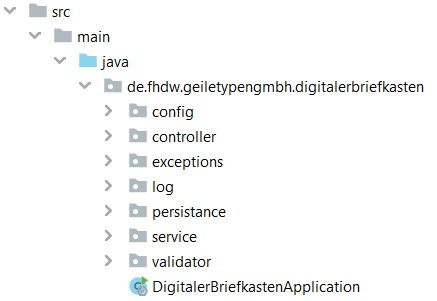
\includegraphics[width=0.5\textwidth]{img/Projekt-root-ordner.png}\\
        \source{Eigene Darstellung}
        \label{fig:root-ordner}
    \end{minipage}
\end{figure}

In dem Projektordner befindet sich der Unterordner \textit{src/main/java/de/fhdw/geiletypengmbh/digitalerbriefkasten}. In diesem
befindet sich der erstellte Quelltext. Die Unterordner (Packages) dessen werden folgend grob erklärt.
\begin{itemize}
    \item config
    \subitem Hierin ist die \textit{SecurityConfig} der Anwendung enthalten.
    \item controller
    \subitem Hierin liegen die Controller. Diese stellen die erreichbaren Endpunkte für die Benutzeroberfläche sowie die REST-API zur Verfügung.
    \item exceptions
    \subitem Hierin befinden sich eigene Exceptions. Diese werden an die Benutzeroberfläche im Fehlerfall weitergeleitet. Ein Beispiel dafür ist die \textit{IdeaNotFoundException}.
    \item log
    \subitem Hierin liegen alle Klassen, die zum Logging von Ereignissen dienen.
    \item persistance
    \subitem Das Package \textit{persistance} dient zum Speichern der Daten (Objekte bzw. Entities) in der Datenbank. Es ist untergliedert
    in die packages
    \begin{itemize}
        \item model
        \subitem Hierin liegen die Datenklassen (Entities). Sie entsprechen dem ER-Diagramm.
        \item repo
        \subitem Hierin liegen die \textit{Repositories}. Sie dienen zum Lesen, Schreiben, etc. der Datenklassen in die Datenbank.
    \end{itemize}
    \item service
    \subitem Hierin liegen die \textit{Services}. Sie dienen als Abstraktionsschicht über den \textit{Repositories}. Damit kann zusätzliche Logik z.B. vor dem Speichern einer Entität implementiert werden. Auch Hilfsmethoden befinden sich in den Services.
    \item validator
    \subitem Hierin liegt die Validationsklasse für die Benutzerstellung. Sie enthält Prüfungen, wie z.B. die Prüfung auf Mindest-Passwortlänge.
\end{itemize}
Darüber hinaus befindet sich in dem Package noch die Hauptklasse der Anwendung \textit{DigitalerBriefkastenApplication}, durch welche sie gestartet wird.
\newline
Neben \textit{src/main/java} existiert auch der Ordner \textit{src/main/resources}. In diesem sind die Komponenten für die Weboberfläche der Anwendung enhalten.
In \cref{fig:resources-ordner} wird die Struktur von \textit{resources} dargestellt.

\begin{figure}[htb]
    \centering
    \begin{minipage}[H]{1\textwidth}
        \caption{Ordnerstruktur der Ressourcen}
        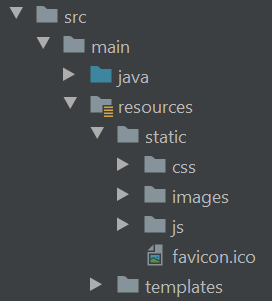
\includegraphics[width=0.5\textwidth]{img/resources-ordner.png}\\
        \source{Eigene Darstellung}
        \label{fig:resources-ordner}
    \end{minipage}
\end{figure}

Der Unterordner \textit{static} beinhaltet css-, Bild- und JavaScript-Dateien. In \textit{Templates} befinden sich die HTML Dateien.
Die Testklassen der Anwendung befinden sich in dem Ordner \textit{src/test/java/de/fhdw/geiletypengmbh/digitalerbriefkasten}.

\subsection{Klassendiagramm}
In \cref{fig:advantage-klassendiagramm} wird die Architektur am Beispiel der Klasse \textit{Advantage} erklärt:

\begin{figure}[htb]
    \centering
    \begin{minipage}[H]{1\textwidth}
        \caption{Klassendiagramm Advantage}
        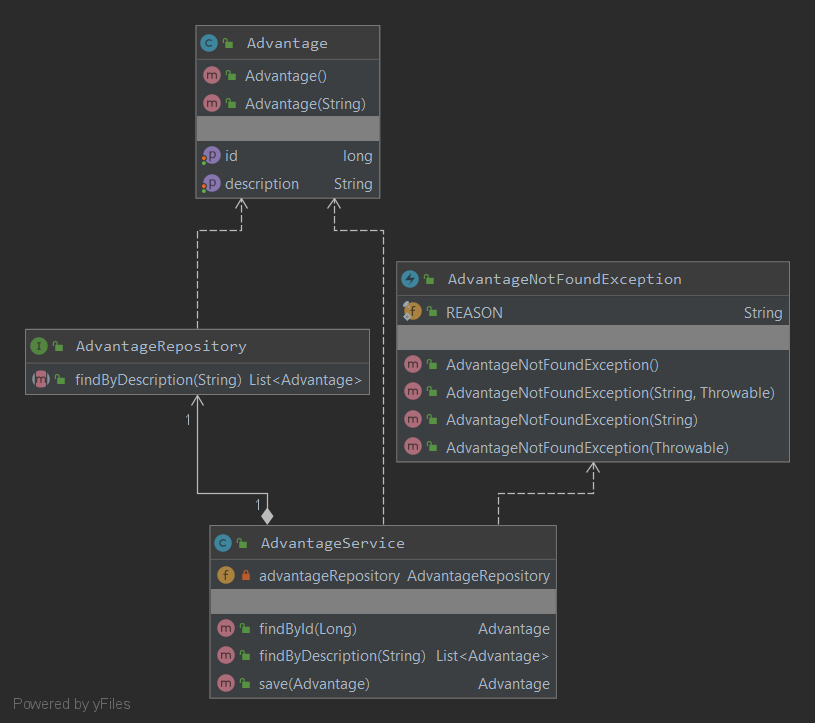
\includegraphics[width=0.75\textwidth]{img/advantage-klassendiagramm.png}\\
        \source{Eigene Darstellung}
        \label{fig:advantage-klassendiagramm}
    \end{minipage}
\end{figure}

Die Klasse \textit{Advantage} stellt die Entität dar, welche von den verschiedenen Schichten der Anwendung verwendet wird.
Das \textit{AdvantageRepository} ist eine Erweiterung des \textit{JPARepositories} und dient somit zur Interaktion mit der Datenbank und Advantage-Objekten.
Darauf aufbauende Logik wird in dem \textit{AdvantageService} implementiert. Dieser wirft zum Beispiel eine \textit{AdvantageNotFoundException} in der
Methode \textit{findById()}, wenn keine Advantage in der Datenbank gefunden wird.
\\
Auf ein Klassendiagramm der gesamten Anwendung wurde verzichtet, da es zu unüberischtlich ist.
In Anhang \ref{Anhang:Klassendiagramme} sind Klassendiagramme des \textit{Models} zu finden, die dem ER-Diagramm entsprechen.



